\documentclass[11pt]{article}

\usepackage[T1]{fontenc}
\usepackage{lmodern}
\usepackage{microtype}
\usepackage[margin=0.92in]{geometry}
\usepackage{amsmath,amssymb,amsthm,mathtools}
\usepackage{booktabs,longtable,array}
\usepackage{enumitem}
\usepackage{graphicx}
\usepackage{xcolor}
\usepackage{tikz}
\usetikzlibrary{arrows.meta,positioning,calc,decorations.pathreplacing,fit}
\usepackage{listings}
\usepackage{hyperref}
\usepackage[nameinlink,noabbrev]{cleveref}
\usepackage{fancyhdr}
\usepackage{caption}
\usepackage{url}

\hypersetup{
  colorlinks=true,
  linkcolor=blue!55!black,
  citecolor=blue!55!black,
  urlcolor=blue!55!black,
  pdftitle={A sign-imbalance strengthened volumetric history adversary for comparison sorting},
  pdfauthor={Nicholas Nash}
}

\setlength{\headheight}{14pt}
\pagestyle{fancy}
\fancyhf{}
\fancyhead[L]{Strengthened-curvature sorting adversary}
\fancyhead[R]{Research checkpoint}
\fancyfoot[C]{\thepage}

\newtheorem{theorem}{Theorem}[section]
\newtheorem{lemma}[theorem]{Lemma}
\newtheorem{proposition}[theorem]{Proposition}
\newtheorem{corollary}[theorem]{Corollary}
\newtheorem{claim}[theorem]{Claim}
\theoremstyle{definition}
\newtheorem{definition}[theorem]{Definition}
\newtheorem{remark}[theorem]{Remark}

\newcommand{\R}{\mathbb{R}}
\newcommand{\diag}{\operatorname{diag}}
\newcommand{\tr}{\operatorname{tr}}
\newcommand{\im}{\operatorname{im}}
\newcommand{\rank}{\operatorname{rank}}
\newcommand{\eps}{\varepsilon}
\newcommand{\PhiV}{\Phi}
\newcommand{\Vnat}{\mathcal{V}}
\newcommand{\Kcert}{\frac{347}{50}}
\newcommand{\Kdecimal}{6.94}
\newcommand{\Ccert}{C_{\mathrm{SI}}}
\newcommand{\ccert}{c_{\mathrm{SI}}}
\newcommand{\norm}[1]{\left\lVert #1\right\rVert}
\newcommand{\ip}[2]{\left\langle #1,#2\right\rangle}
\newcommand{\pos}[1]{\left[#1\right]_+}

\lstset{
  basicstyle=\ttfamily\scriptsize,
  breaklines=true,
  columns=fullflexible,
  frame=single,
  showstringspaces=false,
  language=Python,
  tabsize=4
}

\title{\textbf{A Sign-Imbalance Strengthened Volumetric History Adversary\\for Comparison Sorting}\\[1ex]
\large A carefully audited computer-assisted theorem at coefficient $0.7155799779\ldots$}
\author{Nicholas Nash}
\date{August 29, 2026}

\begin{document}
\maketitle

\begin{abstract}
We give a deterministic polynomial-time adversary for comparison sorting that forces
\[
  \left(0.715579977964088\ldots\right)n\log_2 n-O(n)
\]
comparisons.  The adversary retains the complete directed comparison history and assigns to it the volumetric potential
\[
  \PhiV(G)=\min_{x\in K_G}\frac12\log_2\det\!\left(\sum_i\frac{a_i a_i^{\mathsf T}}{s_i(x)^2}\right).
\]
The initial-to-terminal potential gap is $n\log_2n-O(n)$.  The main theorem is a universal one-comparison estimate
\[
  \min_{\pm}\bigl(\PhiV(G\pm xy)-\PhiV(G)\bigr)
  \le \frac12\log_2\!\left(\frac{347}{50}\right)
  =1.397467831401768\ldots .
\]
After whitening the old Hessian, the second derivative of the augmented log determinant has an exact row-space projection formula.  A new spectral argument shows that curvature is strictly smaller whenever the positive and negative electrical movements are imbalanced.  Integrating this saving, averaging the two answer branches, and proving a sign-separated endpoint reduction leaves a scalar envelope in the normalized query offset $\delta$ and the positive electrical-energy fraction $r$.  A rational piecewise-linear trial schedule and directed-rounding interval arithmetic certify the envelope on $[0,0.411]\times[0,1]$; larger offsets are handled directly at the old center.

The analytic argument and the verification program were independently replayed for this note.  The audit found no substantive mathematical error.  It did identify and repair a formal issue in the first certificate implementation: several already-rounded scalar bounds were combined outside interval arithmetic.  The revised verifier performs the final upper- and lower-bound compositions interval-wise at 120 decimal places and retains a certified natural-log margin of
\[
  4.678410452938429\times 10^{-7}.
\]
\end{abstract}

\begin{center}
\fbox{\begin{minipage}{0.93\linewidth}
\textbf{Status.}  The theorem is exact apart from the usual trusted-implementation assumption for the interval-arithmetic library used by the final finite certificate.  Every combinatorial, matrix-analytic, and scalar-reduction step is proved symbolically.  The rational value $347/50$ is a convenient certified constant; no optimality claim is made for the schedule or for the method.
\end{minipage}}
\end{center}

\tableofcontents

\section{Introduction}

A comparison adversary answers the queries of a sorting algorithm while remaining consistent with at least one total order.  If computational cost is ignored, the adversary can preserve the larger half of the current linear extensions and force $\log_2(n!)=n\log_2n-O(n)$ comparisons.  Efficient deterministic adversaries are more difficult because exact linear-extension counting is \#P-complete~\cite{BrightwellWinkler1991}.

Kaplan, Zamir, and Zwick constructed a deterministic polynomial-time adversary forcing
\[
  \frac{37}{64}n\log_2n=0.578125\,n\log_2n
\]
comparisons~\cite{KaplanZamirZwick2019}.  Their adversary uses a finite interval-lattice state space with local pairing structures.  The history-DAG approach studied here is different: every informative comparison is retained as a linear inequality, including inequalities that later become transitively redundant, and one global log-determinant potential is optimized over the resulting polytope.

The first theorem from this approach used a tangent-plane estimate and gave coefficient
\[
  0.587889382992416\ldots .
\]
Retaining a general second-order term raised the coefficient to
\[
  0.694468130795582\ldots .
\]
The present note exploits additional sign information in that curvature term and proves
\[
  \boxed{0.715579977964088\ldots}.
\]
This is an absolute improvement of $0.1374549779\ldots$ over $37/64$, or approximately $23.78\%$ relatively.  It also exceeds the clean coefficient $5/7$.

\subsection{Proof architecture}
The proof has six layers.
\begin{enumerate}[label=(\roman*)]
  \item The volumetric potential starts at $\frac32n$ and is at least $(n+\frac12)\log_2(n+1)$ when sorting is complete.
  \item At the old volumetric center, whitening turns the old constraint rows into an isotropic frame and the queried comparison into a unit direction.
  \item Along the corresponding electrical direction, the augmented log determinant has an exact projection formula for its second derivative.
  \item The block-diagonal part of a diagonal matrix must be large when its positive and negative eigenvalue norms are unequal.  This gives a new sign-imbalance curvature saving.
  \item After integration, an arbitrary convex average of the two answer branches reduces all frame dependence to the energy split
  \[
    r=\sum_{\alpha_i>0}\alpha_i^2.
  \]
  A convexity lemma shows that only two sign endpoints need be checked.
  \item A fixed rational trial schedule and a two-dimensional interval certificate prove the determinant bound $347/50$.
\end{enumerate}

\subsection{Logarithm convention}
Throughout, $\ln$ is the natural logarithm and $\log$ is $\log_2$.  Determinant ratios are first bounded in natural logarithms.  Since the potential contains one half of a base-$2$ log determinant, a bound $\ln K$ on the relative log determinant gives comparison cost $\frac12\log_2K$.

\section{History polytope and volumetric potential}

Let $V=[n]$ be the items.  The adversary maintains an acyclic directed graph $G=(V,E)$, where $u\to v$ records an informative answer $u<v$.  Edges are never deleted.

For each item $v$, introduce a coordinate $x_v$.  Define the open history polytope
\begin{equation}
  K_G=\left\{x\in\R^n:
  0<x_v<1\ \forall v,\quad x_v-x_u>0\ \forall (u,v)\in E
  \right\}.
  \label{eq:history-polytope}
\end{equation}
Write every inequality as
\[
  a_i^{\mathsf T}x>b_i,
  \qquad
  s_i(x)=a_i^{\mathsf T}x-b_i>0.
\]
The two box rows for $v$ are $(a_i,b_i)=(e_v,0)$ and $(-e_v,-1)$; a comparison $u<v$ contributes $(e_v-e_u,0)$.

The Hessian of the logarithmic barrier is
\begin{equation}
  H_G(x)=\sum_i\frac{a_i a_i^{\mathsf T}}{s_i(x)^2}.
  \label{eq:H}
\end{equation}
The box rows make $H_G(x)$ positive definite throughout $K_G$.  Define
\begin{equation}
  \Vnat_G(x)=\frac12\ln\det H_G(x)
  \label{eq:Vnat}
\end{equation}
and
\begin{equation}
  \boxed{
  \PhiV(G)=\min_{x\in K_G}\frac{\Vnat_G(x)}{\ln2}
  =\min_{x\in K_G}\frac12\log_2\det H_G(x).
  }
  \label{eq:potential}
\end{equation}
The volumetric barrier is convex and tends to $+\infty$ at the relevant boundary faces, so a minimizer exists in the interior.  Standard deterministic convex-optimization machinery approximates its value and center in polynomial time; see Vaidya's volumetric-barrier framework~\cite{Vaidya1996}.

\subsection{Gradient and leverage scores}
At an interior point $x$, define
\begin{equation}
  \sigma_i(x)=\frac{a_i^{\mathsf T}H_G(x)^{-1}a_i}{s_i(x)^2}.
  \label{eq:leverage}
\end{equation}
Differentiation gives
\begin{equation}
  \nabla\Vnat_G(x)
  =-\sum_i\sigma_i(x)\frac{a_i}{s_i(x)}.
  \label{eq:gradient}
\end{equation}
Thus every volumetric center $x^\star$ satisfies
\begin{equation}
  \sum_i\sigma_i(x^\star)\frac{a_i}{s_i(x^\star)}=0.
  \label{eq:center-unwhite}
\end{equation}

\section{The endpoint gap}

\subsection{Initial value}
Initially $E=\varnothing$ and the Hessian is diagonal:
\[
  (H_{G_0}(x))_{vv}=\frac1{x_v^2}+\frac1{(1-x_v)^2}.
\]
Each diagonal entry is minimized at $x_v=1/2$, where it equals $8$.  Hence
\begin{equation}
  \boxed{\PhiV(G_0)=\frac32n.}
  \label{eq:initial}
\end{equation}

\subsection{Terminal lower bound}
Suppose the transcript has determined
\[
  v_1<v_2<\cdots<v_n.
\]
Every adjacent relation $v_j<v_{j+1}$ must have been compared directly: a directed path of length at least two would contain an item strictly between two adjacent elements of the final order.

Select only
\[
  0<x_{v_1},\qquad
  x_{v_{j+1}}-x_{v_j}>0\ (1\le j<n),\qquad
  x_{v_n}<1.
\]
Let the slacks be
\begin{equation}
  s_0=x_{v_1},\qquad
  s_j=x_{v_{j+1}}-x_{v_j}\ (1\le j<n),\qquad
  s_n=1-x_{v_n}.
  \label{eq:path-slacks}
\end{equation}
Then $s_j>0$ and $\sum_{j=0}^n s_j=1$.

\begin{lemma}[Path determinant]
The Hessian of these $n+1$ selected rows satisfies
\begin{equation}
  \det H_{\mathrm{path}}
  =\left(\prod_{j=0}^n s_j^{-2}\right)
   \left(\sum_{j=0}^n s_j^2\right).
  \label{eq:pathdet}
\end{equation}
\end{lemma}

\begin{proof}
Contract the fixed boundary points $0$ and $1$ to one ground vertex.  The selected rows become a weighted cycle with edge weights $w_j=s_j^{-2}$, and $H_{\mathrm{path}}$ is its reduced weighted Laplacian.  The weighted matrix-tree theorem gives
\[
  \det H_{\mathrm{path}}
  =\sum_{j=0}^n\prod_{k\ne j}w_k
  =\left(\prod_{k=0}^n w_k\right)\left(\sum_{j=0}^n\frac1{w_j}\right),
\]
which is \cref{eq:pathdet}.
\end{proof}

AM--GM and Cauchy--Schwarz imply
\[
  \prod_{j=0}^n s_j\le(n+1)^{-(n+1)},
  \qquad
  \sum_{j=0}^n s_j^2\ge\frac1{n+1}.
\]
Therefore
\[
  \det H_{\mathrm{path}}\ge(n+1)^{2n+1}.
\]
The full terminal Hessian dominates this positive-definite path Hessian, so determinant monotonicity yields
\begin{equation}
  \boxed{
  \PhiV(G_T)\ge\left(n+\frac12\right)\log_2(n+1).
  }
  \label{eq:terminal}
\end{equation}
Combining \cref{eq:initial,eq:terminal}, the required potential increase is $n\log_2n-O(n)$.

\section{Whitened geometry of one comparison}

Fix a current history $G$, a volumetric center $x^\star$, and an informative query with normal
\[
  q=e_y-e_x.
\]
Write
\begin{equation}
  H=H_G(x^\star),
  \qquad
  R=q^{\mathsf T}H^{-1}q.
  \label{eq:R}
\end{equation}
Orient $q$ so that $q^{\mathsf T}x^\star\ge0$, and define the normalized offset
\begin{equation}
  \delta=\frac{q^{\mathsf T}x^\star}{\sqrt R}\ge0.
  \label{eq:delta}
\end{equation}

Whiten the old Hessian:
\begin{equation}
  c=\frac{H^{-1/2}q}{\sqrt R},
  \qquad
  u_i=\frac{H^{-1/2}a_i}{s_i(x^\star)}.
  \label{eq:whiten}
\end{equation}
Then
\begin{equation}
  \norm{c}=1,
  \qquad
  \sum_i u_i u_i^{\mathsf T}=I.
  \label{eq:isotropy}
\end{equation}
Set
\begin{equation}
  \alpha_i=u_i^{\mathsf T}c,
  \qquad
  \sigma_i=\norm{u_i}^2.
  \label{eq:alphasigma}
\end{equation}
If $U$ is the matrix with rows $u_i^{\mathsf T}$, then $UU^{\mathsf T}$ is an orthogonal projection.  Consequently
\begin{equation}
  0\le\sigma_i\le1,
  \qquad
  \alpha_i^2\le\sigma_i,
  \qquad
  \sum_i\alpha_i^2=1.
  \label{eq:frame-identities}
\end{equation}
Taking the inner product of \cref{eq:center-unwhite} with $H^{-1/2}q/\sqrt R$ gives
\begin{equation}
  \boxed{\sum_i\sigma_i\alpha_i=0.}
  \label{eq:center-alpha}
\end{equation}

Define the unit electrical displacement in the original coordinates by
\begin{equation}
  d=\frac{H^{-1}q}{\sqrt R}.
  \label{eq:direction}
\end{equation}
Moving from $x^\star$ to $x^\star+s d$ changes the old slacks as
\begin{equation}
  s_i(x^\star+s d)=s_i(x^\star)(1+s\alpha_i)
  \label{eq:slack-move}
\end{equation}
and changes the query coordinate to
\begin{equation}
  q^{\mathsf T}(x^\star+s d)=\sqrt R(\delta+s).
  \label{eq:query-move}
\end{equation}
Because $|\alpha_i|\le1$, every displacement $|s|<1$ preserves all old inequalities.

\begin{figure}[t]
\centering
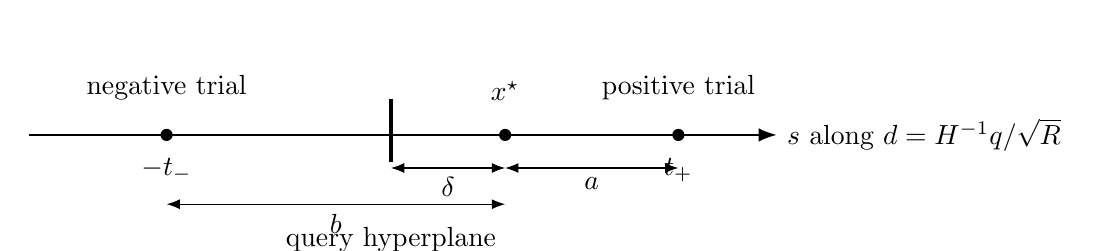
\begin{tikzpicture}[scale=1.0,>=Latex]
  \draw[->,thick] (-4.6,0)--(4.9,0) node[right] {$s$ along $d=H^{-1}q/\sqrt R$};
  \draw[very thick] (0,-0.35)--(0,0.45);
  \node[below=30pt] at (0,0) {query hyperplane};
  \fill (1.45,0) circle (2.2pt);
  \node[above=9pt] at (1.45,0) {$x^\star$};
  \fill (3.65,0) circle (2.2pt);
  \node[above=9pt] at (3.65,0) {positive trial};
  \fill (-2.85,0) circle (2.2pt);
  \node[above=9pt] at (-2.85,0) {negative trial};
  \node[below=5pt] at (-2.85,0) {$-t_-$};
  \node[below=5pt] at (3.65,0) {$t_+$};
  \draw[<->] (0,-0.42)--(1.45,-0.42) node[midway,below] {$\delta$};
  \draw[<->] (1.45,-0.42)--(3.65,-0.42) node[midway,below] {$a$};
  \draw[<->] (-2.85,-0.88)--(1.45,-0.88) node[midway,below] {$b$};
\end{tikzpicture}
\caption{The old center and the two electrical trial points.  The displacement magnitudes are $a$ and $b$, while the final normalized query slacks are $t_+=\delta+a$ and $t_-=b-\delta$.}
\label{fig:trials}
\end{figure}

For a fixed prospective query slack $t>0$, define
\begin{equation}
  A(s)=\sum_i\frac{u_i u_i^{\mathsf T}}{(1+s\alpha_i)^2},
  \qquad
  M_t(s)=A(s)+\frac{cc^{\mathsf T}}{t^2},
  \qquad
  F_t(s)=\ln\det M_t(s).
  \label{eq:Fdef}
\end{equation}
The query row is held fixed during this interpolation; only the endpoint needs to correspond to a genuine trial point.  At $s=0$,
\begin{equation}
  F_t(0)=\ln(1+t^{-2}).
  \label{eq:F0}
\end{equation}
If the positive trial uses displacement $a$ and final slack $t_+=\delta+a$, then $F_{t_+}(a)$ is exactly the natural log of its Hessian determinant relative to the old determinant.  Similarly, $F_{t_-}(-b)$ is the relative log determinant of the negative trial when $t_-=b-\delta>0$.

\section{Exact curvature and the sign-imbalance saving}

\subsection{Projection formula for the second derivative}
At interpolation position $s$, form the augmented row matrix whose first row is $c^{\mathsf T}/t$ and whose remaining rows are $u_i^{\mathsf T}/(1+s\alpha_i)$.  Denote it by $V_s$, so
\[
  M_t(s)=V_s^{\mathsf T}V_s.
\]
Define
\begin{equation}
  P_s=V_sM_t(s)^{-1}V_s^{\mathsf T},
  \qquad
  Q_s=I-P_s,
  \label{eq:PQ}
\end{equation}
so that $P_s$ is the orthogonal projection onto the column space of $V_s$.  Also define
\begin{equation}
  D_s=\diag\!\left(0,\frac{\alpha_1}{1+s\alpha_1},\ldots,
  \frac{\alpha_m}{1+s\alpha_m}\right).
  \label{eq:Ds}
\end{equation}
The leading zero corresponds to the fixed query row.

Differentiating row scales gives
\[
  M_t'(s)=-2V_s^{\mathsf T}D_sV_s,
  \qquad
  M_t''(s)=6V_s^{\mathsf T}D_s^2V_s.
\]
Therefore
\begin{equation}
  F_t''(s)
  =6\tr(P_sD_s^2)-4\tr(P_sD_sP_sD_s).
  \label{eq:Fpp-projection}
\end{equation}
Let
\begin{equation}
  T_s=\norm{P_sD_sP_s}_F^2,
  \qquad
  W_s=\norm{Q_sD_sQ_s}_F^2.
  \label{eq:TW}
\end{equation}
Writing $D_s$ in blocks relative to $\im P_s\oplus\ker P_s$ shows
\begin{equation}
  \boxed{
  F_t''(s)=3\norm{D_s}_F^2-T_s-3W_s.
  }
  \label{eq:Fpp-exact}
\end{equation}
Indeed, if the off-diagonal block has squared Frobenius norm $B_s$, then the right side and \cref{eq:Fpp-projection} both equal $2T_s+6B_s$.

\subsection{A spectral lower bound on the block-diagonal part}
Let
\begin{equation}
  p_s=\left(\sum_{\alpha_i>0}\frac{\alpha_i^2}{(1+s\alpha_i)^2}\right)^{1/2},
  \qquad
  n_s=\left(\sum_{\alpha_i<0}\frac{\alpha_i^2}{(1+s\alpha_i)^2}\right)^{1/2}.
  \label{eq:psns}
\end{equation}
These are the Euclidean norms of the positive and negative eigenvalues of the diagonal matrix $D_s$.

\begin{lemma}[Sign-imbalance lemma]
For every $s$ for which \cref{eq:Fdef} is defined,
\begin{equation}
  \boxed{T_s+W_s\ge\frac12(p_s-n_s)^2.}
  \label{eq:imbalance}
\end{equation}
\end{lemma}

\begin{proof}
Put
\[
  X=P_sD_sP_s+Q_sD_sQ_s,
  \qquad
  Y=P_sD_sQ_s+Q_sD_sP_s.
\]
Then $D_s=X+Y$ and
\[
  \norm{X}_F^2=T_s+W_s.
\]
Relative to $\im P_s\oplus\ker P_s$, the matrix $Y$ has block form
\[
  Y=\begin{pmatrix}0&B\\B^{\mathsf T}&0\end{pmatrix}.
\]
Its nonzero eigenvalues occur in pairs $+\mu_j,-\mu_j$.  Hence the positive and negative eigenvalue vectors of $Y$ have the same Euclidean norm, say $z$.

Hoffman--Wielandt gives
\[
  \norm{D_s-Y}_F^2
  \ge \norm{\lambda(D_s)-\lambda(Y)}_2^2,
\]
where eigenvalues are listed in monotone order.  Separating positive and negative coordinates and padding with zeros if necessary, the right side is at least
\[
  (p_s-z)^2+(n_s-z)^2
  \ge \frac12(p_s-n_s)^2.
\]
Since $D_s-Y=X$, this proves \cref{eq:imbalance}.
\end{proof}

Combining \cref{eq:Fpp-exact,eq:imbalance} gives the central analytic improvement.

\begin{theorem}[Strengthened curvature inequality]
For every $|s|<1$,
\begin{equation}
  \boxed{
  F_t''(s)
  \le
  3\sum_i\frac{\alpha_i^2}{(1+s\alpha_i)^2}
  -\frac12(p_s-n_s)^2.
  }
  \label{eq:strengthened-curvature}
\end{equation}
The bound is independent of the fixed query slack $t$.
\end{theorem}

\begin{proof}
Equation \cref{eq:Fpp-exact} implies
\[
  F_t''(s)
  \le 3\norm{D_s}_F^2-(T_s+W_s).
\]
Apply \cref{eq:imbalance} and expand $\norm{D_s}_F^2$.
\end{proof}

\begin{remark}
Discarding the final term in \cref{eq:strengthened-curvature} recovers the curvature estimate behind the earlier $0.694468\ldots$ checkpoint.  The new term is substantial precisely when positive and negative electrical movements carry unequal squared mass.
\end{remark}

\section{Integrating the curvature bound}

\subsection{The first derivative}
Let
\begin{equation}
  m_3=\sum_i\alpha_i^3.
  \label{eq:m3}
\end{equation}
Since
\[
  M_t(0)^{-1}=I-\frac{cc^{\mathsf T}}{1+t^2},
\]
we obtain
\begin{align}
  F_t'(0)
  &=-2\sum_i\alpha_i\left(\sigma_i-\frac{\alpha_i^2}{1+t^2}\right)\\
  &=-2\sum_i\sigma_i\alpha_i+\frac{2}{1+t^2}\sum_i\alpha_i^3.
\end{align}
Using \cref{eq:center-alpha},
\begin{equation}
  \boxed{F_t'(0)=\frac{2m_3}{1+t^2}.}
  \label{eq:Fprime0}
\end{equation}

\subsection{Energy split and lower bounds on the saving}
Define
\begin{equation}
  r=\sum_{\alpha_i>0}\alpha_i^2,
  \qquad
  P=\sqrt r,
  \qquad
  N=\sqrt{1-r}.
  \label{eq:rPN}
\end{equation}
For $s\ge0$,
\begin{equation}
  p_s\ge\frac{P}{1+sP},
  \qquad
  n_s\le\frac{N}{1-sN}.
  \label{eq:pnbounds}
\end{equation}
The first inequality uses $0<\alpha_i\le P$ on the positive sign class; the second uses $0<-\alpha_i\le N$ on the negative class.

If $N\ge P$, then positive movement makes the negative part more dominant, and
\begin{equation}
  n_s-p_s\ge N-P.
  \label{eq:constant-gap}
\end{equation}
If $P>N$, then
\begin{equation}
  |p_s-n_s|
  \ge
  \pos{\frac{P}{1+sP}-\frac{N}{1-sN}}.
  \label{eq:cross-gap}
\end{equation}
The expression inside the positive part vanishes at
\begin{equation}
  s_0=\frac{P-N}{2PN},
  \label{eq:s0}
\end{equation}
with the natural interpretation $s_0=+\infty$ when $N=0$.

For a positive displacement $a\in(0,1)$ define the certified saving
\begin{equation}
  \Gamma_+(a;r)=
  \begin{cases}
  \displaystyle \frac{a^2}{4}(N-P)^2,&N\ge P,\\[2.5ex]
  \displaystyle \frac12\int_0^{\min(a,s_0)}(a-s)
  \left(\frac{P}{1+sP}-\frac{N}{1-sN}\right)^2\,ds,&P>N.
  \end{cases}
  \label{eq:Gamma-plus}
\end{equation}
For a negative displacement $b\in(0,1)$, reflection $\alpha_i\mapsto-\alpha_i$ gives
\begin{equation}
  \Gamma_-(b;r)=\Gamma_+(b;1-r).
  \label{eq:Gamma-minus}
\end{equation}
These are lower bounds on the integrated contribution of the final term in \cref{eq:strengthened-curvature}.

\subsection{The two branch inequalities}
For any scalar $u>-1$,
\begin{equation}
  \int_0^a(a-s)\frac{\alpha^2}{(1+s\alpha)^2}\,ds
  =a\alpha-\ln(1+a\alpha).
  \label{eq:basic-integral}
\end{equation}
Choose positive and negative trial displacements $a,b\in(0,1)$ with $b>\delta$, and set
\begin{equation}
  t_+=\delta+a,
  \qquad
  t_-=b-\delta.
  \label{eq:tpm}
\end{equation}
Integrating \cref{eq:strengthened-curvature} twice and using \cref{eq:F0,eq:Fprime0,eq:basic-integral} yields
\begin{equation}
  F_{t_+}(a)
  \le \ln(1+t_+^{-2})+\sum_i\phi_+(\alpha_i)-\Gamma_+(a;r),
  \label{eq:positive-branch}
\end{equation}
where
\begin{equation}
  \phi_+(x)=\frac{2a}{1+t_+^2}x^3+3\bigl(ax-\ln(1+ax)\bigr),
  \label{eq:phi-plus}
\end{equation}
and
\begin{equation}
  F_{t_-}(-b)
  \le \ln(1+t_-^{-2})+\sum_i\phi_-(\alpha_i)-\Gamma_-(b;r),
  \label{eq:negative-branch}
\end{equation}
where
\begin{equation}
  \phi_-(x)=-\frac{2b}{1+t_-^2}x^3+3\bigl(-bx-\ln(1-bx)\bigr).
  \label{eq:phi-minus}
\end{equation}

\section{A sign-separated endpoint reduction}

Take any averaging parameter $\lambda\in[0,1]$ and define
\begin{equation}
  \phi_\lambda(x)=\lambda\phi_+(x)+(1-\lambda)\phi_-(x).
  \label{eq:phi-lambda}
\end{equation}
Because the smaller branch is no larger than every convex combination,
\begin{align}
  \min\{F_{t_+}(a),F_{t_-}(-b)\}
  \le{}&\lambda\ln(1+t_+^{-2})+(1-\lambda)\ln(1+t_-^{-2})\notag\\
  &+\sum_i\phi_\lambda(\alpha_i)
  -\lambda\Gamma_+(a;r)-(1-\lambda)\Gamma_-(b;r).
  \label{eq:convex-average}
\end{align}
No algorithmic randomization is involved: $\lambda$ is only a proof witness.

Define
\begin{equation}
  \rho_\lambda(x)=\frac{\phi_\lambda(x)}{x^2}\quad(x\ne0),
  \qquad
  \rho_\lambda(0)=\frac32\bigl(\lambda a^2+(1-\lambda)b^2\bigr).
  \label{eq:rho}
\end{equation}

\begin{lemma}[Endpoint reduction on each sign class]
For $P=\sqrt r$ and $N=\sqrt{1-r}$,
\begin{equation}
  \sup_{0\le x\le P}\rho_\lambda(x)
  =\max\{\rho_\lambda(0),\rho_\lambda(P)\},
  \label{eq:endpoint-positive}
\end{equation}
while
\begin{equation}
  \sup_{-N\le x\le0}\rho_\lambda(x)
  =\max\{\rho_\lambda(0),\rho_\lambda(-N)\}.
  \label{eq:endpoint-negative}
\end{equation}
\end{lemma}

\begin{proof}
For $x>0$, use
\[
  ax-\ln(1+ax)=a^2x^2\int_0^1\frac{z}{1+axz}\,dz
\]
and
\[
  -bx-\ln(1-bx)=b^2x^2\int_0^1\frac{z}{1-bxz}\,dz.
\]
After differentiating $\rho_\lambda$, every nonconstant derivative term is a positive multiple of one of
\[
  q_+(u)=-\int_0^1\frac{z^2}{(1+uz)^2}\,dz,
  \qquad
  q_-(u)=\int_0^1\frac{z^2}{(1-uz)^2}\,dz.
\]
Both functions are increasing on their domains.  Hence $\rho_\lambda'$ is increasing on $(0,P]$, so $\rho_\lambda$ is convex there and its maximum on $[0,P]$ is attained at an endpoint.  Applying the same argument to $y\mapsto\rho_\lambda(-y)$ proves the negative statement.
\end{proof}

Since every positive $\alpha_i$ lies in $(0,P]$ and every negative one lies in $[-N,0)$, \cref{eq:endpoint-positive,eq:endpoint-negative} gives
\begin{equation}
  \sum_i\phi_\lambda(\alpha_i)
  \le rM_+(\delta,r;a,b,\lambda)+(1-r)M_-(\delta,r;a,b,\lambda),
  \label{eq:frame-reduction}
\end{equation}
where
\begin{align}
  M_+&=\max\{\rho_\lambda(0),\rho_\lambda(\sqrt r)\},\\
  M_-&=\max\{\rho_\lambda(0),\rho_\lambda(-\sqrt{1-r})\}.
\end{align}

Define the final scalar envelope
\begin{align}
  \mathcal B(\delta,r;a,b,\lambda)
  ={}&\lambda\ln\!\left(1+\frac1{(\delta+a)^2}\right)
  +(1-\lambda)\ln\!\left(1+\frac1{(b-\delta)^2}\right)\notag\\
  &+rM_++(1-r)M_-\notag\\
  &-\lambda\Gamma_+(a;r)-(1-\lambda)\Gamma_-(b;r).
  \label{eq:B}
\end{align}
Equations \cref{eq:convex-average,eq:frame-reduction} prove
\begin{equation}
  \min\{F_{t_+}(a),F_{t_-}(-b)\}
  \le\mathcal B(\delta,r;a,b,\lambda).
  \label{eq:B-bounds-F}
\end{equation}
Thus the arbitrary-dimensional comparison problem has been reduced exactly to two state variables, $\delta$ and $r$, plus three proof choices $a,b,\lambda$.

\section{The certified trial schedule}

Set
\begin{equation}
  K=\Kcert=6.94,
  \qquad
  D_0=\frac1{\sqrt{K-1}}=0.410304969931109\ldots .
  \label{eq:KD0}
\end{equation}
For $0\le\delta\le0.411$, use the rational piecewise-linear schedule listed in \cref{tab:schedule}.  Between consecutive knots, $a(\delta)$ and $b(\delta)$ are linearly interpolated.  Every displayed decimal is an exact rational with denominator $10^9$; every $\delta$ knot has denominator $1000$.

\begin{longtable}{@{}r r r r r@{}}
\caption{Certified trial schedule.  Here $t_+=\delta+a$ and $t_-=b-\delta$.}
\label{tab:schedule}\\
\toprule
$\delta$ & $a$ & $b$ & $t_+$ & $t_-$\\
\midrule
\endfirsthead
\toprule
$\delta$ & $a$ & $b$ & $t_+$ & $t_-$\\
\midrule
\endhead
0.000&0.622454434&0.622424669&0.622454434&0.622424669\\
0.020&0.619095674&0.625535911&0.639095674&0.605535911\\
0.040&0.615380539&0.628496630&0.655380539&0.588496630\\
0.060&0.611228294&0.631313547&0.671228294&0.571313547\\
0.080&0.606581110&0.633952170&0.686581110&0.553952170\\
0.100&0.601325567&0.636408839&0.701325567&0.536408839\\
0.120&0.595325316&0.638653695&0.715325316&0.518653695\\
0.140&0.588378953&0.640666245&0.728378953&0.500666245\\
0.160&0.580204170&0.642417260&0.740204170&0.482417260\\
0.180&0.570394627&0.643880998&0.750394627&0.463880998\\
0.200&0.558360320&0.645041599&0.758360320&0.445041599\\
0.220&0.543240708&0.645950414&0.763240708&0.425950414\\
0.240&0.523955919&0.647234041&0.763955919&0.407234041\\
0.260&0.503631525&0.627425532&0.763631525&0.367425532\\
0.280&0.484458268&0.576626027&0.764458268&0.296626027\\
0.300&0.465515284&0.602315113&0.765515284&0.302315113\\
0.320&0.446808252&0.631351002&0.766808252&0.311351002\\
0.340&0.428343050&0.660180668&0.768343050&0.320180668\\
0.360&0.410125825&0.707228286&0.770125825&0.347228286\\
0.380&0.392162933&0.690669770&0.772162933&0.310669770\\
0.400&0.374460973&0.732158061&0.774460973&0.332158061\\
0.410&0.365700000&0.750000000&0.775700000&0.340000000\\
0.411&0.364823903&0.751784194&0.775823903&0.340784194\\
\bottomrule
\end{longtable}

The schedule satisfies
\[
  0<a(\delta)<1,
  \qquad
  \delta<b(\delta)<1,
\]
throughout the certified range, so both old-constraint trial displacements and both final query slacks are feasible.

\begin{figure}[t]
\centering
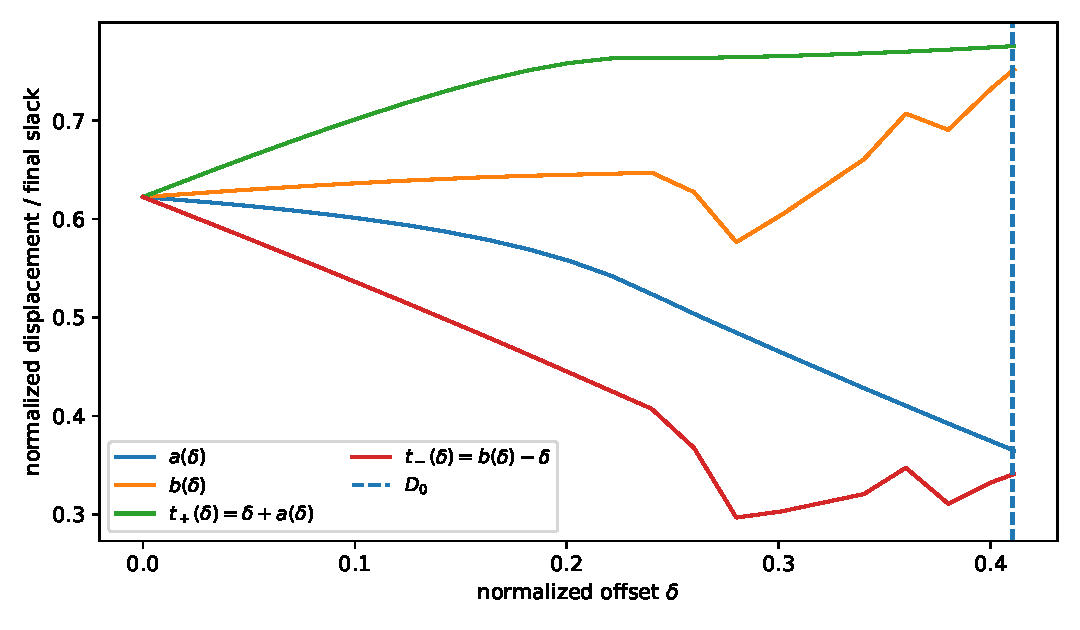
\includegraphics[width=0.88\linewidth]{schedule_plot.pdf}
\caption{The rational piecewise-linear displacement schedule and the resulting final query slacks.  The dashed line marks the direct large-offset threshold $D_0$.}
\label{fig:schedule}
\end{figure}

\begin{theorem}[Certified scalar envelope]
For every $0\le\delta\le0.411$ and every $0\le r\le1$, there exists $\lambda\in[0,1]$ such that the schedule in \cref{tab:schedule} satisfies
\begin{equation}
  \boxed{
  \mathcal B(\delta,r;a(\delta),b(\delta),\lambda)<\ln\!\left(\frac{347}{50}\right).
  }
  \label{eq:certificate-theorem}
\end{equation}
\end{theorem}

\begin{proof}
This is the finite interval certificate described in \cref{sec:certificate-details}.  The complete revised verification source accompanies this note.
\end{proof}

\subsection{Large offsets}
When $\delta\ge D_0$, evaluate the answer branch containing the old center at $x^\star$.  The old Hessian is unchanged and the new query row has normalized slack $\delta$.  The matrix-determinant lemma gives
\begin{equation}
  \frac{\det H_{\mathrm{new}}(x^\star)}{\det H}
  =1+\delta^{-2}
  \le1+D_0^{-2}=K.
  \label{eq:large-offset}
\end{equation}
Since $D_0<0.411$, the near- and large-offset arguments overlap.

\section{Universal comparison theorem and global adversary}

\begin{theorem}[One-comparison determinant bound]
For every current history and every informative comparison, one of the two consistent answers satisfies
\begin{equation}
  \frac{\det H_{\mathrm{new}}(z)}{\det H_G(x^\star)}\le\frac{347}{50}
  \label{eq:det-ratio-main}
\end{equation}
for an explicit feasible trial point $z$ in that answer branch.  Consequently,
\begin{equation}
  \boxed{
  \min_{\pm}\bigl(\PhiV(G\pm xy)-\PhiV(G)\bigr)
  \le\frac12\log_2\!\left(\frac{347}{50}\right).
  }
  \label{eq:comparison-cost}
\end{equation}
\end{theorem}

\begin{proof}
If $\delta\le0.411$, apply \cref{eq:B-bounds-F,eq:certificate-theorem}; the smaller of the two trial log determinants is less than $\ln K$.  If $\delta\ge D_0$, use \cref{eq:large-offset}.  These ranges cover all $\delta\ge0$.  Since each branch potential is the minimum over its feasible points, it is no larger than the corresponding trial value.  Dividing the relative natural log determinant by $2\ln2$ proves \cref{eq:comparison-cost}.
\end{proof}

Define
\begin{equation}
  \Ccert=\frac12\log_2\!\left(\frac{347}{50}\right)
  =1.39746783140176810589\ldots
  \label{eq:Ccert}
\end{equation}
and
\begin{equation}
  \ccert=\frac1{\Ccert}
  =\frac{2}{\log_2(347/50)}
  =0.71557997796408866862\ldots .
  \label{eq:ccert}
\end{equation}

\begin{theorem}[Main adversary theorem]
There is a deterministic polynomial-time adversary that forces every comparison sorting algorithm to perform at least
\begin{equation}
  \boxed{
  \frac{
  \left(n+\frac12\right)\log_2(n+1)-\frac32n-O(n^{-2})
  }{
  \frac12\log_2(347/50)
  }
  }
  \label{eq:finite-main}
\end{equation}
informative comparisons, and therefore at least
\begin{equation}
  \boxed{
  \left(0.715579977964088\ldots\right)n\log_2n-O(n)
  }
  \label{eq:asymptotic-main}
\end{equation}
total comparisons.
\end{theorem}

\begin{proof}
On an informative query, approximate the two child potentials to additive accuracy $n^{-4}$ and choose the smaller approximation.  The chosen true potential is at most the smaller true child potential plus $2n^{-4}$.  There are at most $\binom n2$ informative unordered pairs, so the total decision error is $O(n^{-2})$.

If $Q$ informative comparisons occur, \cref{eq:comparison-cost} and telescoping give
\[
  \PhiV(G_T)-\PhiV(G_0)
  \le \Ccert Q+O(n^{-2}).
\]
Use \cref{eq:initial,eq:terminal} and rearrange.  Repeated or already implied queries only increase the sorting algorithm's total comparison count and do not weaken the lower bound.
\end{proof}

\section{Polynomial-time implementation}

At every stage the state has at most $2n+\binom n2=O(n^2)$ inequalities, all with coefficients in $\{-1,0,1\}$.  A topological ordering $v_1,\ldots,v_n$ of the current DAG gives the explicit interior point
\[
  x_{v_j}=\frac{j}{n+1},
\]
whose box and comparison slacks are at least $1/(n+1)$.  The polytope lies in a Euclidean ball of radius $\sqrt n$.  Thus the domain has polynomially bounded inner and outer radii in the standard bit model.

The objective $\Vnat_G(x)=\frac12\ln\det H_G(x)$, its gradient, and separation from the domain boundary can be evaluated to polynomial precision using rational linear algebra and standard high-precision arithmetic.  Deterministic convex optimization therefore yields an additive $n^{-4}$ approximation in time polynomial in $n$.  The adversary computes the two child values on each informative query and answers according to the smaller approximation.  No certificate variables $a,b,r,$ or $\lambda$ are needed by the adversary; they exist only in the proof of the universal transition bound.

\section{Certificate details and audit}
\label{sec:certificate-details}

\subsection{Box decomposition and rational witnesses}
The certificate covers
\[
  (\delta,r)\in\left[0,\frac{411}{1000}\right]\times[0,1].
\]
Each interval between consecutive $\delta$ knots in \cref{tab:schedule} is initially divided into ten equal rational pieces; $[0,1]$ in $r$ is divided into one hundred equal pieces.  A box that does not certify immediately is split into four equal subboxes.  The final run used
\[
  27{,}166\ \text{accepted boxes},\qquad
  1{,}722\ \text{split nodes},\qquad
  \text{maximum depth }4.
\]

For each box, ordinary floating point is used only to propose a value of $\lambda$.  It is rounded to an exact rational with denominator $10^{12}$.  That fixed rational is then evaluated over the entire box with interval arithmetic.  Correctness does not depend on the floating-point proposal succeeding optimally: if the proposed witness is poor, the box simply fails and is subdivided.

\subsection{Interval upper bounds}
For a given box, $\delta$, $a(\delta)$, and $b(\delta)$ are interval quantities constructed from exact rational endpoints.  The two query-row terms in \cref{eq:B} are evaluated directly with outward-rounded intervals.

For fixed $\delta,a,b,\lambda$, the function $\rho_\lambda$ is convex on each sign interval.  Hence over every $r$ in a box $[r_0,r_1]$,
\[
  \sup_{0\le x\le\sqrt r}\rho_\lambda(x)
  \le\max\{\rho_\lambda(0),\rho_\lambda(\sqrt{r_1})\},
\]
and
\[
  \sup_{-\sqrt{1-r}\le x\le0}\rho_\lambda(x)
  \le\max\{\rho_\lambda(0),\rho_\lambda(-\sqrt{1-r_0})\}.
\]
After these two scalar bounds are fixed, the mixture $rM_++(1-r)M_-$ is affine in $r$, so its maximum occurs at $r_0$ or $r_1$.

\subsection{Interval lower bounds on the savings}
The saving in \cref{eq:Gamma-plus} is monotone in the displacement length.  On the side $P>N$, it can be written
\[
  \frac12\int_0^a(a-s)
  \left[\frac{P}{1+sP}-\frac{N}{1-sN}\right]_+^2ds.
\]
For $P=\sqrt r$ and $N=\sqrt{1-r}$, the integrand is pointwise nondecreasing in $r$ on $[1/2,1]$.  Therefore a certified lower bound over an $r$-box uses the displacement lower endpoint and the $r$ endpoint closest to $1/2$.  The reflected rule applies on $[0,1/2]$.  If a box straddles $1/2$, the program safely discards both nonnegative savings.

The cross-over integral is evaluated by the exact elementary antiderivative in \cref{app:gamma-closed-form}.  Every final upper/lower composition in the revised verifier is itself performed with interval operations.

\subsection{Certificate output}
At 120 decimal places, the revised verifier reports
\begin{align*}
  \ln(347/50)&\ge
  1.9373017745187131337349260584753076874674754\ldots,\\
  \max\mathcal B&\le
  1.9373013066776678398920256287059302483882368\ldots.
\end{align*}
The certified margin is
\begin{equation}
  \boxed{
  0.0000004678410452938429004297693774390792386\ldots>0.
  }
  \label{eq:margin}
\end{equation}
The largest certified box was
\[
  \delta\in[0.210,0.211],
  \qquad
  r\in[0.940,0.945],
\]
with rational witness
\[
  \lambda=\frac{489435582914}{10^{12}}.
\]
The direct threshold satisfies
\[
  D_0<0.411,
\]
so there is no gap between the certified and large-offset regimes.

\begin{figure}[t]
\centering
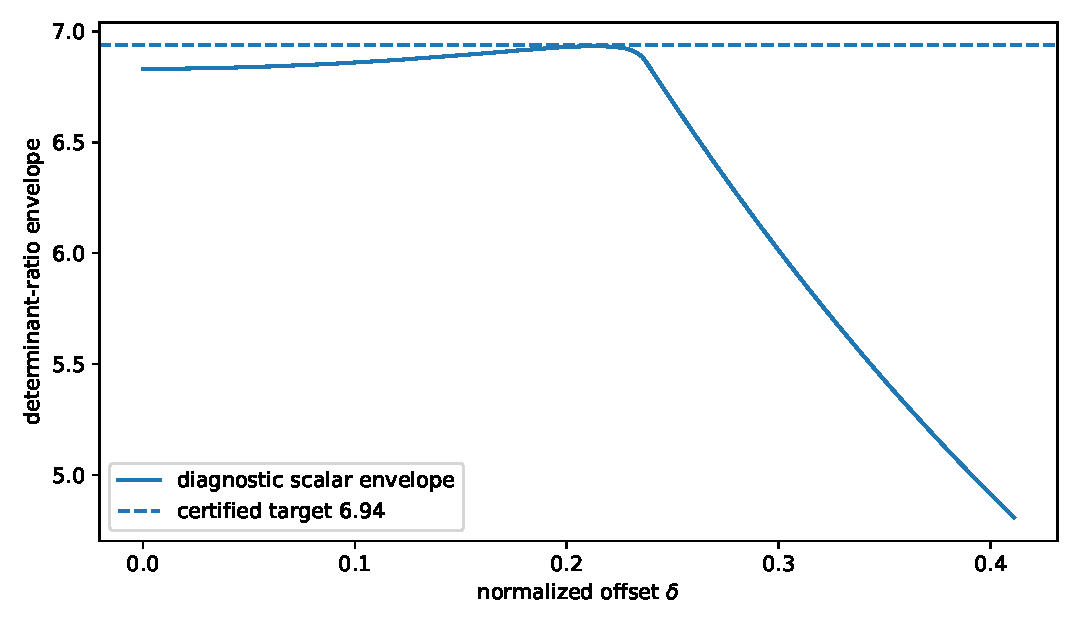
\includegraphics[width=0.86\linewidth]{diagnostic_envelope_plot.pdf}
\caption{A dense floating-point scan of the optimized scalar envelope.  This plot is diagnostic only; the theorem uses the interval certificate.  The scan's maximum determinant ratio is about $6.93397$, while interval dependency enlarges the certified worst upper bound to just below $6.94$.}
\label{fig:diagnostic-envelope}
\end{figure}

\subsection{Audit replay}
The following checks were performed independently of the original derivation.
\begin{enumerate}[label=(\alph*)]
  \item The endpoint determinant identity, gradient formula, whitening identities, and both trial-point Hessians were re-derived symbolically.
  \item The exact formulas \cref{eq:Fpp-projection,eq:Fpp-exact} were recomputed from $F_t(s)=\ln\det M_t(s)$.
  \item The sign-imbalance lemma was checked against random finite-dimensional projections; all sampled slacks were positive, and the two formulas for $F_t''$ agreed to approximately $8\times10^{-15}$ in double precision.
  \item The closed form for the cross-over saving was compared with independent high-precision quadrature at fifty random points; the largest double-precision discrepancy was below $8\times10^{-17}$.
  \item A $207\times501$ dense scan of $(\delta,r)$, independently optimizing the scalar $\lambda$ witness, found maximum determinant envelope approximately $6.93396948$ near $\delta=0.2155$, $r=0.936$.  This is diagnostic, not part of the proof.
  \item The revised interval verifier was rerun at both 120 and 170 decimal places.  It produced the same subdivision tree, maximum box, and certified margin to all displayed digits.
\end{enumerate}
The diagnostic source and transcript accompany the note.

\subsection{Correction to the first verifier}
The first $6.94$ script already used 90-place interval arithmetic for all transcendental expressions and had a margin of roughly $4.68\times10^{-7}$.  However, a few already-rounded scalar upper and lower bounds were subsequently multiplied or added in the ordinary \texttt{mpmath} scalar context.  At 90 digits this could not plausibly consume the numerical margin, but it was an avoidable formal weakness.

The revised verifier:
\begin{itemize}
  \item raises both scalar and interval precision to 120 decimal places;
  \item constructs all theorem constants, domain endpoints, and schedule values from integers;
  \item performs the $r$-mixture, squared lower endpoints, correction combination, and final upper-bound composition through interval operations;
  \item compares a certified upper bound for each box with a certified lower bound for $\ln(347/50)$;
  \item checks feasibility and overlap with the large-offset regime explicitly.
\end{itemize}
The source SHA-256 is
\begin{center}
\texttt{cf30be0c7d87db6e3ed4b1192aba5742843757c90cbea0596c2e4f4227a29570}.
\end{center}

\subsection{Trusted implementation boundary}
The finite certificate relies on the outward-rounding behavior of \texttt{mpmath.iv}.  The proof does not rely on ordinary floating point except to suggest rational witnesses that are subsequently certified.  A future archival version would ideally replay the same boxes in a second interval system based on MPFR or Arb.  This is a software-assurance improvement, not a known mathematical gap.

\section{Interpretation and remaining slack}

The previous curvature proof used only
\[
  F_t''(s)\le3\norm{D_s}_F^2.
\]
The present argument subtracts at least
\[
  \frac12(p_s-n_s)^2.
\]
This explains the qualitative jump from $0.694468\ldots$ to $0.715579\ldots$: the old scalar worst cases placed most electrical energy on one sign, exactly where the discarded curvature was largest.

The certificate's hardest region is moderately offset and strongly imbalanced:
\[
  \delta\approx0.21,
  \qquad
  r\approx0.94.
\]
The target is not tight for centered queries, and the rational schedule is visibly nonoptimal in places.  Further progress could come from a sharper spectral distance than \cref{eq:imbalance}, a richer summary than the single sign-energy parameter $r$, or an analytic optimization of the scalar schedule.  None of these refinements is needed for the theorem proved here.

\section{Conclusion}

The enriched history-DAG volumetric method now gives a deterministic polynomial-time adversary forcing
\[
  \boxed{
  \left(0.715579977964088\ldots\right)n\log_2n-O(n)
  }
\]
comparisons.  The principal new idea is that the exact row-space curvature formula remembers the positive/negative imbalance of electrical row motions.  Once this information is retained, the high-dimensional comparison transition reduces to a certified two-variable scalar problem.

The result is computer-assisted only in the final compact optimization.  The proof reduction is exact, the schedule is rational, the certificate has a positive directed-rounded margin, and an audited verifier and diagnostic replay accompany this document.

\appendix

\section{Closed form for the cross-over saving}
\label{app:gamma-closed-form}
Assume $P>N>0$, let
\[
  L=\min\left\{\ell,\frac{P-N}{2PN}\right\},
  \qquad
  U=1+PL,
  \qquad
  V=1-NL.
\]
Define
\begin{align*}
  T_1&=(P\ell+1)(1-U^{-1})-\ln U,\\
  T_2&=(N\ell-1)(V^{-1}-1)-\ln V,\\
  J_1&=\frac{(P\ell+1)\ln U-(U-1)}{P^2},\\
  J_2&=\frac{-(N\ell-1)\ln V+(1-V)}{N^2},\\
  J_3&=\frac{P}{P+N}J_1+\frac{N}{P+N}J_2.
\end{align*}
Then
\begin{equation}
  \frac12\int_0^L(\ell-s)
  \left(\frac{P}{1+sP}-\frac{N}{1-sN}\right)^2ds
  =\frac12\left(T_1+T_2-2PNJ_3\right).
  \label{eq:Gamma-closed}
\end{equation}
For $N=0$, the continuous limit is
\begin{equation}
  \frac12\left((P\ell+1)\left(1-\frac1{1+P\ell}\right)-\ln(1+P\ell)\right).
  \label{eq:Gamma-N0}
\end{equation}
These are the formulas evaluated by the verifier.

\section{Numerical constants}
\begin{align*}
  K&=\frac{347}{50}=6.94,\\
  \ln K&=1.9373017745187131337349260584753076874674754\ldots,\\
  \frac12\log_2K&=1.3974678314017681058914091175738851307014079\ldots,\\
  \frac{2}{\log_2K}&=0.7155799779640886686282167598910260395514797\ldots,\\
  D_0&=\frac1{\sqrt{K-1}}=0.4103049699311091091141355337508101186113234\ldots.
\end{align*}

\section{Revised certificate transcript}
\begin{lstlisting}[language={}]
PASS
K [6.93999999999999999999999999999999999999999999999999...,
   6.94000000000000000000000000000000000000000000000000...]
target [1.93730177451871313373492605847530768746747543351662...,
        1.93730177451871313373492605847530768746747543351663...]
D0 [0.41030496993110910911413553375081011861132343872350...,
    0.41030496993110910911413553375081011861132343872351...]
cover 0.411
cells 27166 splits 1722 depth 4
maxub 1.9373013066776678398920256287059302483882368152883195
margin 0.0000004678410452938429004297693774390792386182283063
coefficient [0.71557997796408866862821675989102603955147970028172...,
             0.71557997796408866862821675989102603955147970028173...]
max box delta=[0.210,0.211], r=[0.940,0.945]
lambda=489435582914/10^12
\end{lstlisting}

\section{Accompanying files}
The research bundle contains:
\begin{itemize}
  \item \texttt{strengthened\_curvature\_sorting\_adversary.tex};
  \item the compiled PDF;
  \item \texttt{verify\_0715579\_strengthened\_curvature\_revised.py};
  \item \texttt{certificate\_0715579\_revised.txt};
  \item \texttt{audit\_diagnostics.py} and its output;
  \item the schedule and diagnostic plots.
\end{itemize}

\begin{thebibliography}{99}

\bibitem{KaplanZamirZwick2019}
H.~Kaplan, O.~Zamir, and U.~Zwick,
\newblock A sort of an adversary,
\newblock in \emph{Proceedings of the Thirtieth Annual ACM--SIAM Symposium on Discrete Algorithms (SODA 2019)}, SIAM, 2019, pp.~1291--1310.

\bibitem{Vaidya1996}
P.~M. Vaidya,
\newblock A new algorithm for minimizing convex functions over convex sets,
\newblock \emph{Mathematical Programming}, 73 (1996), pp.~291--341.

\bibitem{BrightwellWinkler1991}
G.~Brightwell and P.~Winkler,
\newblock Counting linear extensions is \#P-complete,
\newblock in \emph{Proceedings of the 23rd Annual ACM Symposium on Theory of Computing}, 1991, pp.~175--181.

\end{thebibliography}

\end{document}
